% !TeX root = ../praktikum.tex
% !TeX encoding = UTF-8
% !Tex spellcheck = de_DE

Um ein Verständnis von Photodioden zu erlangen und da kommerzielle Powermeter mit recht hohen Anschaffungskosten einher gehen, wurde in diesem Versuchsteil versucht, eine Leistungsmessung des Laserlichtes mit Hilfe einer Photodiode aufzunehmen.\\

Die verwendete Photodiode\footnote{Modell OSD15-5T von CENTRONIC\cite{farnell.com_osd15-5t_????}} produziert laut Datenblatt einen Strom von \unit[0,18-0,21]{mA} pro Milliwatt eingestrahlter Lichtleistung bei \unit[436]{nm} Wellenlänge. Da Strom nicht direkt gemessen werden kann, wird ein Widerstand parallel geschaltet und der Spannungsabfall über diesen nach $U=R\cdot I$ mit einem Oszilloskop gemessen. Wenn man für \unit[1]{mW} Lichtleistung einen Spannungsabfall von \unit[100]{mV} erreichen möchte, würde man einen $ \nicefrac{U}{I}=\nicefrac{\unit[100]{mV}}{\unit[0,2]{mA}}=\unit[500]{\ohm}$ Widerstand verwenden. Je kleiner die Spannung ist, desto größer werden die relativen Messfehler, daher wurden \unit[4]{V} pro Milliwatt angesetzt und entsprechend ein \unit[20]{k\ohm} Widerstand verwendet.\\

Bei sehr schwachem Lichteinfall (Deckenlampe, Fenster aus der Ferne, ...) konnte auf dem Oszilloskop eine Schwankung in der Spannung festgestellt werden. Bei höheren Lichtleistungen konnte jedoch auch bei relativ großen Lichtintensitätsschwankungen nur sehr kleine Spannungsveränderungen beobachtet werden. Für andere Widerstandswerte, z.B. \unit[10]{k\ohm} oder \unit[100]{k\ohm}, erhielt man nahezu identische Werte um \unit[440]{mV}. Da dies in etwa der Bandlücke eines PN-Überganges entspricht, liegt die Vermutung nahe, dass dies eine Sättigungserscheinung war.

\begin{figure}[ht]
	\centering
	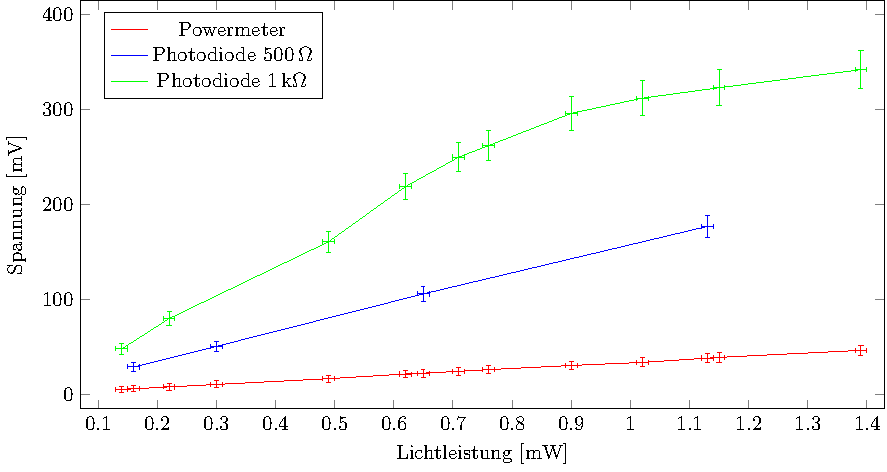
\includegraphics[width=1\linewidth]{graphs/fotodiode/diode.pdf}
	\caption[Vermessung einer Photodiode]{
		Spannungen gemessen über je einen zu einer Photodiode parallel geschalteten Widerstand mit \unit[500]{\ohm} und \unit[1000]{\ohm}. Zusätzlich ist der Verlauf der Spannung eines Powermeters aufgetragen.
	}
	\label{fig:photodiode}
\end{figure}

Daher wurde der Aufbau mit kleineren Widerstandswerten von \unit[500]{\ohm} und \unit[1000]{\ohm} getestet. Die gemessenen Spannungen sowie die dazu vom Powermeter abgelesenen Werte für die Lichtleistung sind in Abbildung~\ref{fig:photodiode} aufgetragen.

Es ist für \unit[1]{\ohm} eine Sättigung ab etwa \unit[0,9]{mW} erkennbar, die Variante mit \unit[500]{\ohm} weist im gesamten Messbereich ein lineares Verhalten auf. Die Fehlerbalken in der x-Achse wurden zu \unit[0,01]{mW} gewählt, da das verwendete Powermeter nur zwei Nachkommastellen in der Einheit \unit{mW} anzeigte. Der Fehler in der y-Achse wurde auf etwa 5\% gewählt.

%Bei dieser Wellenlänge hat die Photodiode eine Effizienz von etwa \unit[20]{\%} bei der Umwandlung von Licht zu Strom. Bei \unit[660]{nm} (Frequenz des Lasers) etwa \unit[40]{\%}.

\subsubsection*{Auswertung}

Um aus dem Spannungsabfall über den zu der Photodiode parallel geschalteten Widerstand eine Lichtleistung bestimmen zu können ist ein lineares Verhalten von Vorteil. So kann direkt aus der Spannung mittels eines Faktors die Leistung berechnet werden. Mit einem Widerstand von \unit[1]{k\ohm} ist ein lineares Verhalten nur im Bereich bis etwa \unit[0,7]{mW} zu beobachten. Darüber hinaus sättigt die Spannung. Mit Hilfe eines kommerziellen Powermeters ließe sich eine Wertetabelle der Spannung gegen die Leistung erstellen, die es erlauben würde auch weit über diesen Bereich hinaus die Lichtleistung berechnen, da auch hier noch eine geringe (jedoch nicht lineare) Zunahme der Spannung zu beobachten war. In diesem Bereich ist jedoch von einem deutlich größerem Fehler auszugehen.

Für den \unit[500]{\ohm} Widerstand ist bis zur maximal vermessenen Lichtleistung $P_L$ von etwa \unit[1,1]{mW} keine Sättigung festzustellen (vgl. Abb.~\ref{fig:photodiode}). Für den vorgesehen Verwendungszweck empfiehlt sich daher die Verwendung eines Widerstandswertes in der Nähe von \unit[500]{\ohm}. Mit Hilfe der Software \textit{QtiPlot} wurde eine Lineare Regression mit der Formel $U=a\cdot P_L + b$ über die aufgenommenen Datenpunkte ausgeführt. Daraus ergeben sich die Werte $b=(5,235 \pm 1,152) \unit{mW} $ und $a=(152,661\pm 1,710) \unitfrac{W}{V}$. Die Standardabweichung liegt bei $1,28$.\\


Das beobachtete Verhalten lässt sich erklären, indem man einen PN-Übergang in der Photodiode mit einer Bandlücke von etwa \unit[400-500]{mV} annimmt. Für eine feste Frequenz kann die Lichtleistung direkt in die Anzahl der Photonen $N_{Ph}$ umgerechnet werden: $N_{Ph} = \nicefrac{P_L}{E_{Ph}}$, wobei $E_{Ph}=\hbar \omega_{Ph}$ die Energie pro Photon ist. Jedes dieser Photonen treibt mit einer Wahrscheinlichkeit, entsprechend der Quanteneffizienz des Überganges für die Frequenz der Photonen $\omega_{Ph}$, genau einen elektronischen Übergang. Bei kleinen Lichtintensitäten und gutem Stromfluss (kleinem Widerstand) kann von einer kompletter Besetzung des unteren Zustandes und einem leeren oberen Zustand ausgegangen werden, da die angeregten Elektronen schnell zurück in den unteren Zustand gelangen können. Es findet daher fast ausschließlich spontane Absorption statt und es werden eine zu der Anzahl der eingestrahlten Photonen proportionale Anzahl Elektronen angeregt. So kommt es zu einem zu der Lichtleistung proportionalen Strom. Der über den Widerstand abfallende Strom ist also proportional zu der eingestrahlten Lichtleistung. Dies erklärt das lineare Verhalten bei kleinen Widerständen beziehungsweise geringen Lichtleistungen.\\
Sobald dieser Widerstand jedoch relativ zur Lichtleistung so groß gewählt wird, dass der Spannungsabfall in etwa dem Bandlückenpotential entspricht, erhöht sich die Anzahl der besetzen Zustände im oberen Zustand. Dadurch findet neben spontaner Absorption auch stimulierte Emission statt. Das Verhältnis zwischen Photonen und angeregten Elektronen ändert sich. Folglich sinkt die abgefallene Spannung über den Widerstand. Die erklärt das Sättigungsverhalten ab etwa \unit[300]{mV}.
